\documentclass{beamer}
\usepackage{bbm}
\usepackage{algorithm}
\usepackage{algpseudocode}
\usepackage{tikz}
\usepackage{amsmath}
\usepackage{amssymb}
\usepackage{array}
\usepackage{graphicx}
\graphicspath{{figures/}} % Added to ensure the figures directory is searched
\usepackage{capt-of} % Added to enable captionof in beamer

% Theme choice:
\usetheme{Madrid}

% Title page details:
\title{A Petri Nets Model for Blockchain Analysis}
\subtitle{Seminar for the course of CMCS}
\author{Luca Lombardo}
\date{}

\begin{document}

\begin{frame}[plain]
    \titlepage
    \begin{center}
        \footnotesize{\textit{Based on the work of: Andrea Pinna, Roberto Tonelli, Matteo Orr\'{u}, Michele Marchesi}}
    \end{center}
\end{frame}

% Outline frame
\begin{frame}{Structure of the Presentation}
    \tableofcontents
\end{frame}

\section{Introduction: A Petri Net Model for Blockchain Analysis}
\label{sec:Intro}
\begin{frame}{A Petri Net Model for Blockchain Analysis}
    \footnotesize

    \begin{block}{Key Contributions}
        \begin{itemize}
            \item \textbf{Addresses Petri Net (APN):} Maps Bitcoin addresses to \textit{places} and transactions to \textit{transitions} in a P/T Net
            \item \textbf{Entities Petri Net (EPN):} Groups addresses into owner entities using a clustering algorithm
        \end{itemize}
    \end{block}

    \vspace{-0.2cm}
    \begin{block}{Advantages of PN Formalism}
        \begin{itemize}
            \item Algebraic structure enables formal analysis of transaction patterns
            \item Native representation of blockchain architecture through PN semantics
            \item Enables dynamic simulations for network behavior forecasting
        \end{itemize}
    \end{block}

    \vspace{-0.2cm}
    \begin{columns}[T]
        \begin{column}{0.5\textwidth}
            \textbf{Model Features}
            \begin{itemize}
                \item Preserves transaction topology
                \item Supports address clustering
                \item Enables multi-scale analysis
            \end{itemize}
        \end{column}

        \begin{column}{0.5\textwidth}
            \textbf{Paper Structure}
            \begin{itemize}
                \item System overview
                \item PN model definition
                \item APN/EPN construction
                \item Blockchain analysis results
            \end{itemize}
        \end{column}
    \end{columns}
\end{frame}

\subsection{Bitcoin Blockchain}
\begin{frame}{Bitcoin Blockchain: Architecture \& Transactions}
    \footnotesize
    \vspace{-0.2cm}
    \begin{block}{Overview}
        \begin{itemize}
            \item \textbf{Distributed Public Ledger:} A global database that stores every validated Bitcoin transaction.
            \item \textbf{Chain of Blocks:} Transactions are grouped into blocks that form an ordered sequence (the Blockchain).
        \end{itemize}
    \end{block}

    \vspace{-0.2cm}
    \begin{block}{Transaction Structure}
        \begin{itemize}
            \item \textbf{Inputs:} Reference previous unspent outputs (UTXOs) from earlier transactions.
            \item \textbf{Outputs:} List one or more addresses (e.g., strings starting with "1" or "4") along with their associated values.
            \item \textbf{UTXO Model:} An address's balance equals the sum of its unspent outputs.
        \end{itemize}
    \end{block}

    \vspace{-0.2cm}
    \begin{block}{User Interaction}
        \begin{itemize}
            \item \textbf{Digital Wallets:} Bitcoin clients store public/private key pairs that manage one or more addresses.
            \item \textbf{Anonymity:} Only addresses are recorded; no personal identity information is required.
        \end{itemize}
    \end{block}
\end{frame}

\begin{frame}{Bitcoin Blockchain: Architecture \& Transactions}
    \centering
    \label{fig:ReteEsempio_1}
    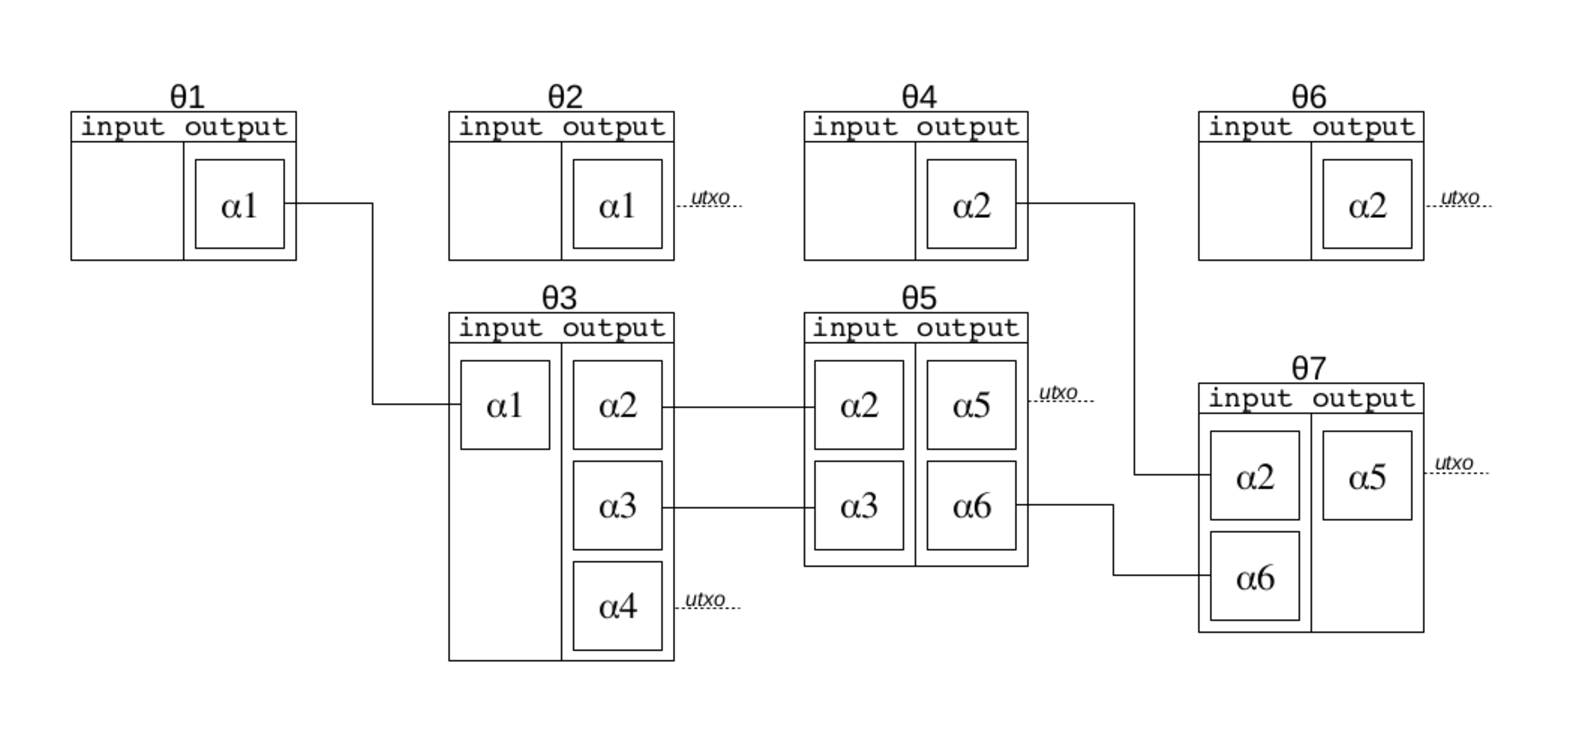
\includegraphics[width=1\linewidth]{ReteEsempio_1}
    \captionof{figure}{Simplified transaction schema}
\end{frame}

\begin{frame}{Bitcoin Blockchain: Transaction Verification \& Mining}
    \footnotesize

    \begin{block}{Transaction Validation}
        \begin{itemize}
            \item \textbf{Broadcast \& Pending:} Transactions are shared in the peer-to-peer network and wait to be validated.
            \item \textbf{Validation Rules:}
                  \begin{itemize}
                      \item Each input must reference a valid UTXO.
                      \item The total value of outputs must not exceed that of inputs.
                  \end{itemize}
        \end{itemize}
    \end{block}

    \begin{block}{Mining Process}
        \begin{itemize}
            \item \textbf{Proof-of-Work:} Miners solve a computational puzzle by finding a hash.
            \item \textbf{Block Contents:} A block includes the selected transactions, the previous block's hash, its block height, and miner information.
            \item \textbf{Incentives:} The first miner to solve the puzzle receives a block reward
        \end{itemize}
    \end{block}
\end{frame}

\subsection{Petri Nets: an overview}
\begin{frame}{Petri Nets: Basic Concepts}
    \footnotesize
    \begin{block}{Overview}
        A \textbf{Petri Net} is a formal model for distributed systems built on a bipartite graph consisting of:
        \begin{itemize}
            \item \textbf{Places:} Represent conditions, resources, or system states.
            \item \textbf{Transitions:} Represent events that change these states.
        \end{itemize}
    \end{block}

    \begin{block}{Graph Structure}
        \begin{itemize}
            \item \textbf{Bipartite Graph:} Only two types of nodes are allowed, and connections occur only between nodes of different types.
            \item \textbf{Arcs:} Directed arcs link places and transitions:
                  \begin{itemize}
                      \item \textit{Pre-arcs:} Arcs from places to transitions (inputs).
                      \item \textit{Post-arcs:} Arcs from transitions to places (outputs).
                  \end{itemize}
        \end{itemize}
    \end{block}
\end{frame}

\begin{frame}{Petri Nets: Algebraic Formalism \& Markings}
    \footnotesize
    \begin{block}{Algebraic Description}
        A Petri Net is formally defined as a quadruple:
        \[
            N = (P, T, Pre, Post)
        \]
        where:
        \begin{itemize}
            \item \(P=\{p_1, p_2, \dots, p_m\}\) is the set of places.
            \item \(T=\{t_1, t_2, \dots, t_n\}\) is the set of transitions.
            \item \(Pre: P \times T \rightarrow \mathbb{N}\) is the \emph{pre-incidence} function.
            \item \(Post: P \times T \rightarrow \mathbb{N}\) is the \emph{post-incidence} function.
        \end{itemize}
        These incidence functions are typically represented as \(m \times n\) matrices.
    \end{block}

\end{frame}

\begin{frame}{Petri Nets: Algebraic Formalism \& Markings}
    \begin{block}{Markings \& Firing Rule}
        \begin{itemize}
            \item A \textbf{marking} \(M\) is a vector assigning tokens to places, thus representing the system state.
            \item \textbf{Firing:} When a transition fires, it:
                  \begin{enumerate}
                      \item Consumes tokens from its pre-connected places.
                      \item Produces tokens in its post-connected places.
                  \end{enumerate}
            \item The complete system is denoted as \(\langle N, \mathbf{M}_0 \rangle\), where \(\mathbf{M}_0\) is the initial marking.
            \item In our work on Blockchain analysis, we focus on the net structure, without defining a specific marking.
        \end{itemize}
    \end{block}

\end{frame}

\section{Address Petri Net}
\begin{frame}{Addresses Petri Net: Overview and Definitions}
    \footnotesize
    \begin{block}{Motivation}
        \begin{itemize}
            \item Blockchain transactions move bitcoins between addresses.
            \item The inherent bipartite structure (addresses and transactions) suggests a natural mapping to a Petri Net.
        \end{itemize}
    \end{block}

    \begin{block}{Definitions}
        \begin{itemize}
            \item \(\mathcal{A}=\{\alpha_1,\alpha_2,\dots,\alpha_m\}\): Finite set of addresses (inputs/outputs).
            \item \(\Theta=\{\theta_1,\theta_2,\dots,\theta_n\}\): Set of validated transactions.
        \end{itemize}
    \end{block}

    \begin{block}{Addresses Petri Net Structure}
        \begin{itemize}
            \item Define \(N_\alpha = (P_{\alpha}, T, \mathbf{PreA}, \mathbf{PostA})\) where:
                  \begin{itemize}
                      \item \(P_{\alpha} = \{p\alpha_1, p\alpha_2, \dots, p\alpha_m\}\) associates one place per address.
                      \item \(T = \{t_1, t_2, \dots, t_n\}\) associates one transition per transaction.
                      \item \(\mathbf{PreA}\) and \(\mathbf{PostA}\) are the pre- and post-incidence matrices.
                  \end{itemize}
            \item These sets are built by scanning the Blockchain for new addresses and transactions.
        \end{itemize}
    \end{block}
\end{frame}

\subsection{Constructing the Incidence Matrices}
\begin{frame}{Addresses Petri Net: Constructing the Incidence Matrices}
    \footnotesize
    \begin{block}{Transaction Representation}
        \begin{itemize}
            \item Each transaction \(\theta\) is split into:
                  \begin{itemize}
                      \item \(\textbf{In}(\theta) \subseteq \mathcal{A}\): Set of input addresses.
                      \item \(\textbf{Out}(\theta) \subseteq \mathcal{A}\): Set of output addresses.
                  \end{itemize}
            \item The corresponding transition \(t\) represents \(\theta\) in the Petri Net.
        \end{itemize}
    \end{block}

    \begin{block}{Matrix Construction}
        \begin{itemize}
            \item For every \(\alpha \in \textbf{In}(\theta)\):
                  \begin{itemize}
                      \item Add a \textbf{pre-arc} from place \(p\alpha\) to transition \(t\).
                      \item Set \(\mathbf{PreA}(p\alpha, t)=1\).
                  \end{itemize}
            \item For every \(\alpha \in \textbf{Out}(\theta)\):
                  \begin{itemize}
                      \item Add a \textbf{post-arc} from transition \(t\) to place \(p\alpha\).
                      \item Set \(\mathbf{PostA}(p\alpha, t)=1\).
                  \end{itemize}
            \item The matrices \(\mathbf{PreA}\) and \(\mathbf{PostA}\) are of dimension \(m\times n\).
        \end{itemize}
    \end{block}
\end{frame}

\begin{frame}{Addresses Petri Net: Example and Analysis}
    \footnotesize
    \vspace{-0.2cm}
    \begin{block}{Example Overview}
        \begin{itemize}
            \item Consider a simplified set of transactions (e.g. as in the previous slide)
            \item The Addresses Petri Net has:
                  \begin{itemize}
                      \item 6 places (\(P_{\alpha} = \{p\alpha_1, \dots, p\alpha_6\}\)).
                      \item 7 transitions (\(T = \{t_1, \dots, t_7\}\)).
                  \end{itemize}
        \end{itemize}
        Below a graphical representation of an addresses Petri Net equivalent to the
        simplified transaction chains.
    \end{block}
    \begin{center}
        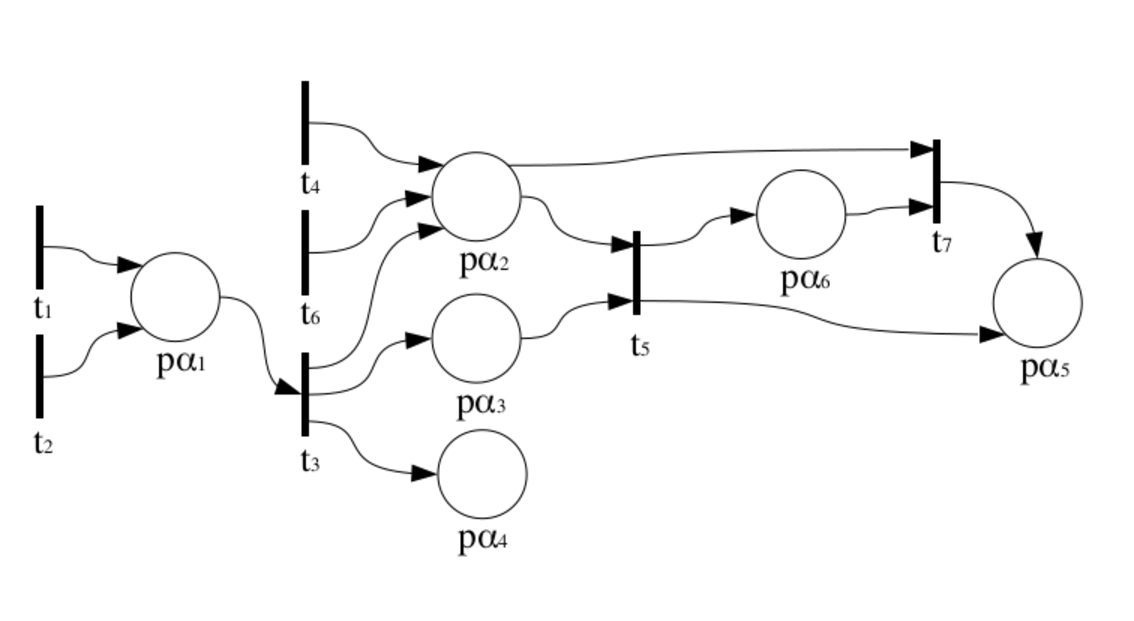
\includegraphics[width=0.7\linewidth]{ReteEsempio_1pt}\label{fig:ReteEsempio_1pt}

    \end{center}

\end{frame}

\begin{frame}
    \frametitle{Address Petri Nets: Incidence Matrices and Analysis}
    \begin{block}{Incidence Matrices and Analysis}
        \begin{itemize}
            \item \textbf{Pre-incidence matrix \(\mathbf{PreA}\):} Captures the number of times an address appears as an input.
            \item \textbf{Post-incidence matrix \(\mathbf{PostA}\):} Captures the outputs associated with each transaction.
            \item By computing the difference (\(\mathbf{PostA} - \mathbf{PreA}\)) for each row, one can:
                  \begin{itemize}
                      \item Determine the number of UTXOs per address.
                      \item Infer whether an address balance is null (zero tokens).
                  \end{itemize}
            \item Transactions sharing identical input and output sets may be merged into one transition with a firing clock, aiding dynamic analyses.
        \end{itemize}
    \end{block}

\end{frame}

\begin{frame}
    \frametitle{Pre-incidence matrix of the simplified transaction}
    \begin{figure}
        \centering{
            \textbf{PreA}=$\begin{bmatrix}
                    0 \  & 0 \  & 1 \  & 0 \  & 0 \  & 0 \  & 0 \\
                    0 \  & 0 \  & 0 \  & 0 \  & 1 \  & 0 \  & 1 \\
                    0 \  & 0 \  & 0 \  & 0 \  & 1 \  & 0 \  & 0 \\
                    0 \  & 0 \  & 0 \  & 0 \  & 0 \  & 0 \  & 0 \\
                    0 \  & 0 \  & 0 \  & 0 \  & 0 \  & 0 \  & 0 \\
                    0 \  & 0 \  & 0 \  & 0 \  & 0 \  & 0 \  & 1 \\
                \end{bmatrix}$
            $\begin{array}{c} p\alpha_1 \\p\alpha_2 \\p\alpha_3 \\p\alpha_4 \\p\alpha_5 \\p\alpha_6 \end{array}
            $\\$\begin{array}{cccccccc}\ \ & t_1 & t_2 & t_3 & t_4 & t_5 & t_6 & t_7 \end{array}$}
        \vspace{.2cm}
        \caption{Pre-incidence matrix of the Petri net for the example of the simplified transaction schema.}
        \label{Pre-esempio1}
    \end{figure}
\end{frame}

\begin{frame}{Post-incidence matrix of the simplified transaction}
    \begin{figure}
        \centering{
            \textbf{PostA}=$\begin{bmatrix}
                    1 \  & 1 \  & 0 \  & 0 \  & 0 \  & 0 \  & 0 \\
                    0 \  & 0 \  & 1 \  & 1 \  & 0 \  & 1 \  & 0 \\
                    0 \  & 0 \  & 1 \  & 0 \  & 0 \  & 0 \  & 0 \\
                    0 \  & 0 \  & 1 \  & 0 \  & 0 \  & 0 \  & 0 \\
                    0 \  & 0 \  & 0 \  & 0 \  & 1 \  & 0 \  & 1 \\
                    0 \  & 0 \  & 0 \  & 0 \  & 1 \  & 0 \  & 0
                \end{bmatrix}$
            $\begin{array}{c} p\alpha_1 \\p\alpha_2 \\p\alpha_3 \\p\alpha_4 \\p\alpha_5 \\p\alpha_6 \end{array}
            $\\ $\begin{array}{cccccccc}\ \ & t_1 & t_2 & t_3 & t_4 & t_5 & t_6 & t_7 \end{array}$}
        \vspace{.2cm}
        \caption{Post-incidence matrix of the Petri net for the example of the simplified transaction schema.}
        \label{Post-esempio1}
    \end{figure}
\end{frame}


\subsection{Entities Petri Net and algorithm to manage them}

\begin{frame}{Entities Petri Net: Introduction}
    \footnotesize
    \begin{block}{Motivation}
        \begin{itemize}
            \item Bitcoin users often control multiple addresses to manage exchanges and preserve anonymity.
            \item We define an \textbf{entity} as the person, organization, or group that controls a set of addresses.
            \item \textbf{Key Property:} All addresses appearing in the input of a single transaction must belong to the same entity
                  (since transferring funds requires control over all associated private keys).
        \end{itemize}
    \end{block}

    \begin{block}{Why Group Addresses?}
        \begin{itemize}
            \item Enables high-level analysis of the Blockchain.
            \item Reduces complexity by clustering addresses that are likely controlled by the same user.
            \item Provides a more natural mapping to real-world economic actors.
        \end{itemize}
    \end{block}
\end{frame}

\begin{frame}{From Addresses to Entities: Definitions \& Mapping}
    \footnotesize
    \begin{block}{Mapping Addresses to Entities}
        \begin{itemize}
            \item Let \(\mathcal{A}=\{\alpha_1, \alpha_2, \dots, \alpha_m\}\) be the set of addresses.
            \item Let \(\Theta=\{\theta_1, \theta_2, \dots, \theta_n\}\) be the set of transactions.
            \item In the Addresses Petri Net \(N_\alpha=(P_\alpha, T, \mathbf{PreA}, \mathbf{PostA})\), each place \(p\alpha\) corresponds to an address \(\alpha\).
        \end{itemize}
    \end{block}

    \begin{block}{Defining an Entity}
        \begin{itemize}
            \item An \textbf{entity} \(\epsilon\) is a set of addresses: \(\epsilon\subseteq \mathcal{A}\).
            \item Denote the set of entities as \(E=\{\epsilon_1, \epsilon_2, \dots, \epsilon_k\}\).
            \item In the \textbf{Entities Petri Net} \(N_{\epsilon}=(P_{\epsilon}, T, \mathbf{PreE}, \mathbf{PostE})\), each place \(p\epsilon\) represents one entity.
        \end{itemize}
    \end{block}
    % In the following slide we will see the Entity Computation Algorithm, whose purpose is to determine which addresses belong to the same entity by examining \(\mathbf{PreA}\).

    % Recall: For each transaction \(t\), the non-zero entries in column \(\mathbf{PreA}(\cdot,t)\) indicate input addresses.
\end{frame}

\begin{frame}[fragile]{}
    \footnotesize
    \begin{algorithm}[H]
        \footnotesize
        \caption{Compute Entities from the Addresses Petri Net}\label{alg:entities}
        \begin{algorithmic}[1]
            \State $T^* \gets T$ \Comment{Set of unexplored transactions}
            \State $E \gets \emptyset$ \Comment{Set of entities}
            \While{$T^* \neq \emptyset$}
            \State Select and remove a transaction $t$ from $T^*$
            \State $e \gets \emptyset$ \Comment{Initialize new entity}
            \ForAll{$p_i$ such that $\mathbf{PreA}(p_i,t)=1$}
            \State $e \gets e \cup \{p_i\}$
            \EndFor
            \State $e^* \gets e$ \Comment{Set of unexplored places within $e$}
            \While{$e^* \neq \emptyset$}
            \State Select a place $p$ from $e^*$
            \ForAll{transactions $t'$ with $\mathbf{PreA}(p,t')=1$}
            \ForAll{$p_h$ such that $\mathbf{PreA}(p_h,t')=1$}
            \State $e \gets e \cup \{p_h\}$, $e^* \gets e^* \cup \{p_h\}$
            \EndFor
            \State Remove $t'$ from $T^*$
            \EndFor
            \State Remove $p$ from $e^*$
            \EndWhile
            \State $E \gets E \cup \{e\}$
            \EndWhile
        \end{algorithmic}
    \end{algorithm}
\end{frame}

\begin{frame}{Entities Petri Net: Incidence Matrices and Aggregation}
    \footnotesize
    \begin{block}{Constructing the Entities Petri Net}
        \begin{itemize}
            \item Each computed entity \(e \in E\) is represented by a unique place \(p\epsilon\) in the Entities Petri Net \(N_{\epsilon}=(P_{\epsilon}, T, \mathbf{PreE}, \mathbf{PostE})\).
            \item The set of transitions \(T\) remains the same as in the Addresses Petri Net.
        \end{itemize}
    \end{block}

    \begin{block}{Aggregating Incidence Matrices}
        \begin{itemize}
            \item For each entity \(e\), identify all corresponding addresses \(p\alpha \in e\) from the Addresses Petri Net.
            \item \(\mathbf{PreE}\) and \(\mathbf{PostE}\) are obtained by summing the rows in \(\mathbf{PreA}\) and \(\mathbf{PostA}\) for all places in \(e\).
            \item This aggregation captures the cumulative input and output interactions of all addresses within the entity.
        \end{itemize}
    \end{block}

    % \begin{block}{Key Benefits}
    %     \begin{itemize}
    %         \item \textbf{Simplification:} Reduces complexity by clustering multiple addresses under a single entity.
    %         \item \textbf{Enhanced Analysis:} Facilitates high-level insights (e.g., UTXO counts and transaction frequencies) by focusing on entity behavior.
    %         \item \textbf{Unified Representation:} Maintains the natural mapping of Blockchain interactions in a concise, algebraic structure.
    %     \end{itemize}
    % \end{block}
\end{frame}

\section{Results}

\begin{frame}{Data Acquisition and Processing Pipeline}
    \footnotesize
    \begin{itemize}
        \item \textbf{Approach:} Downloaded formatted JSON blocks from \textit{blockchain.info}.
        \item \textbf{Dataset:} Parsed the first 180,000 blocks (Jan 2009 -- Mar 2012)
        \item \textbf{Implementation:} Data processing executed in R using RStudio IDE.
        \item \textbf{Performance:} Total processing time $\approx$ 250 hours (avg. 5 sec per block).
    \end{itemize}
    \vspace{0.3cm}
    \centering
    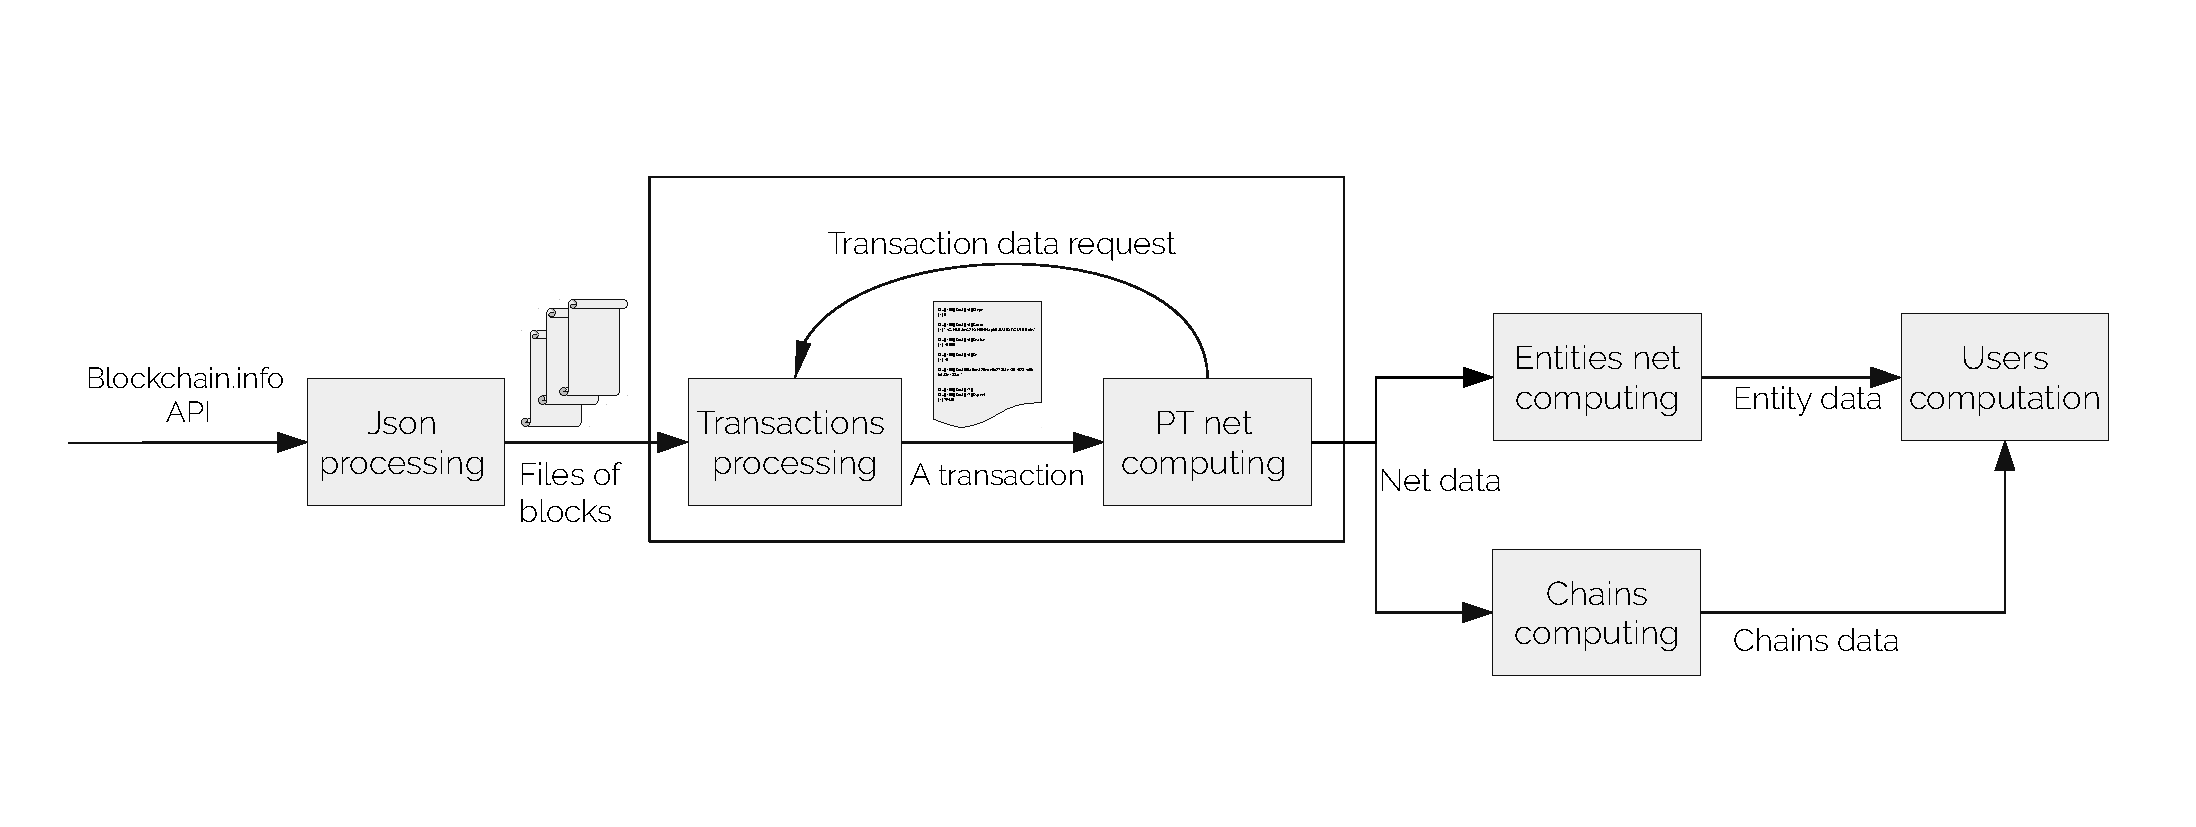
\includegraphics[width=1\linewidth]{diagram}
\end{frame}

\subsection{Results of the Address Petri Net}

\begin{frame}{Addresses Petri Net: Global Statistics and CCDF Analysis}
    \footnotesize
    \begin{itemize}
        \item \textbf{Addresses:} 3,730,480 distinct addresses.
        \item \textbf{Transactions:} 3,142,019 transactions (columns in $\mathbf{PreA}$/$\mathbf{PostA}$).
        \item \textbf{Arcs:} 4,575,888 pre-arcs and 7,352,494 post-arcs.
        \item The number of nonzero elements in a row of $\mathbf{PreA}$ (or $\mathbf{PostA}$) indicates the number of input (or output) transactions for that address.
        \item CCDF plots reveal a power-law distribution: many addresses with few transactions and a few addresses with very high activity.
    \end{itemize}
    \vspace{-0.1cm}
    \begin{minipage}[c]{0.45\textwidth}
        \centering
        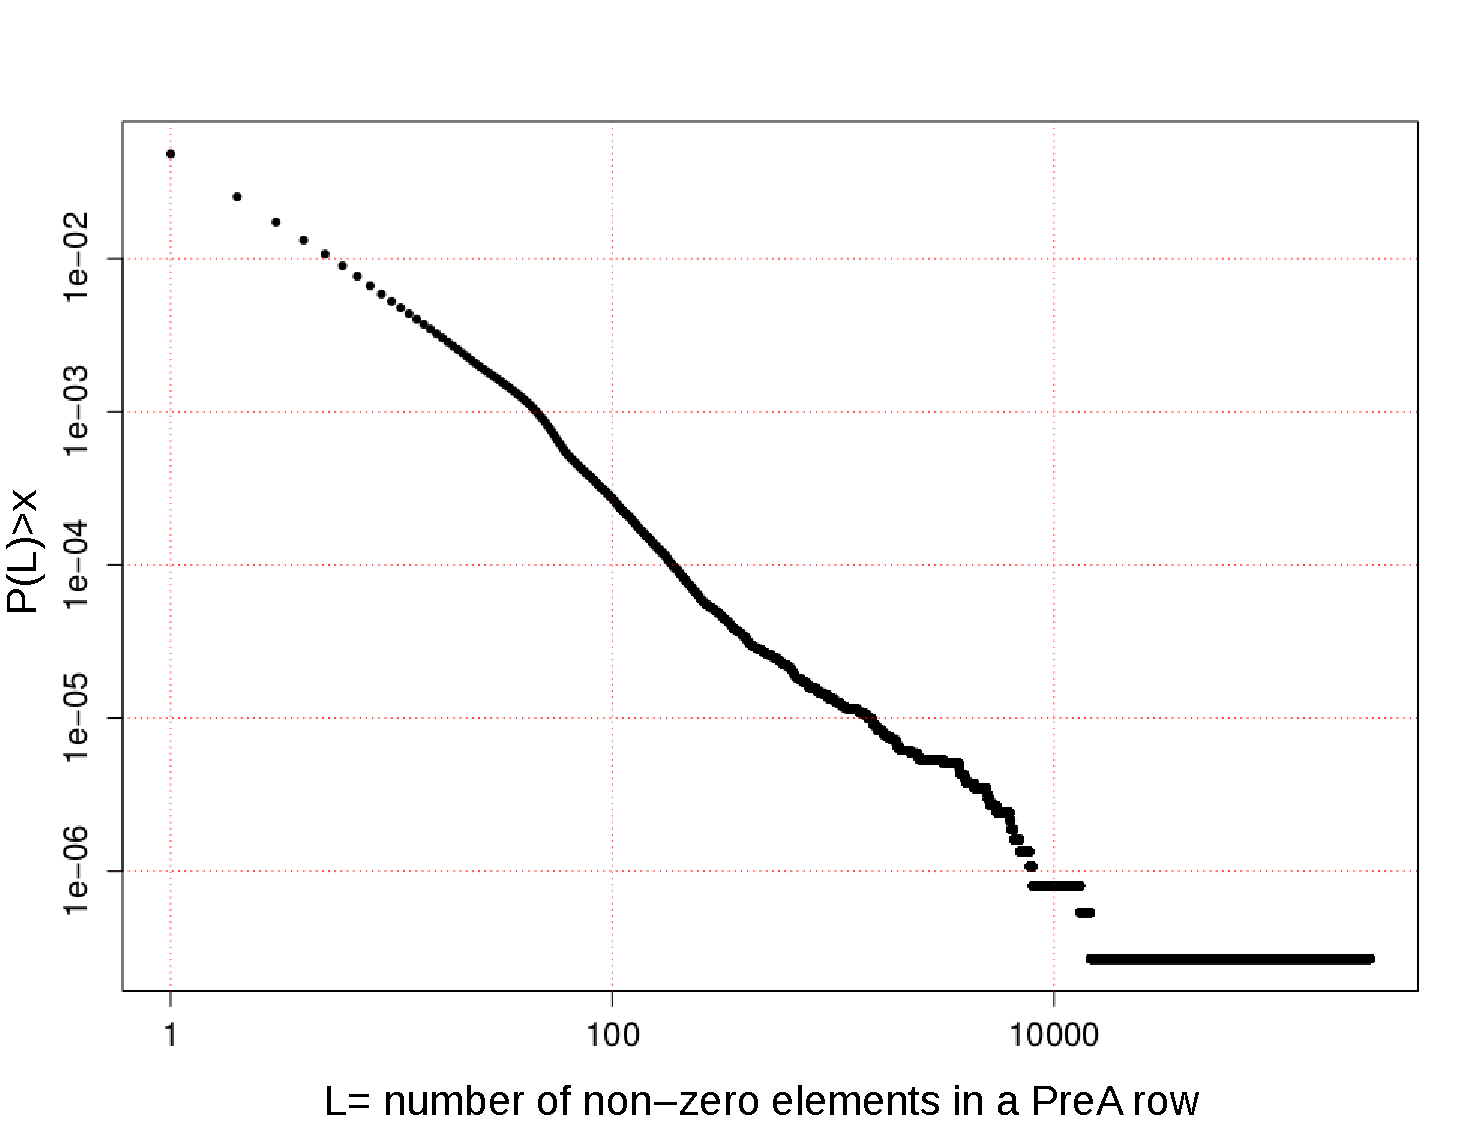
\includegraphics[width=0.95\linewidth]{PreA}
        \footnotesize
        \captionof{figure}{CCDF of $L$ for $\mathbf{PreA}$.}
        \label{fig_preA_CCDF}
    \end{minipage}
    \hspace{0.5cm}
    \begin{minipage}[c]{0.45\textwidth}
        \centering
        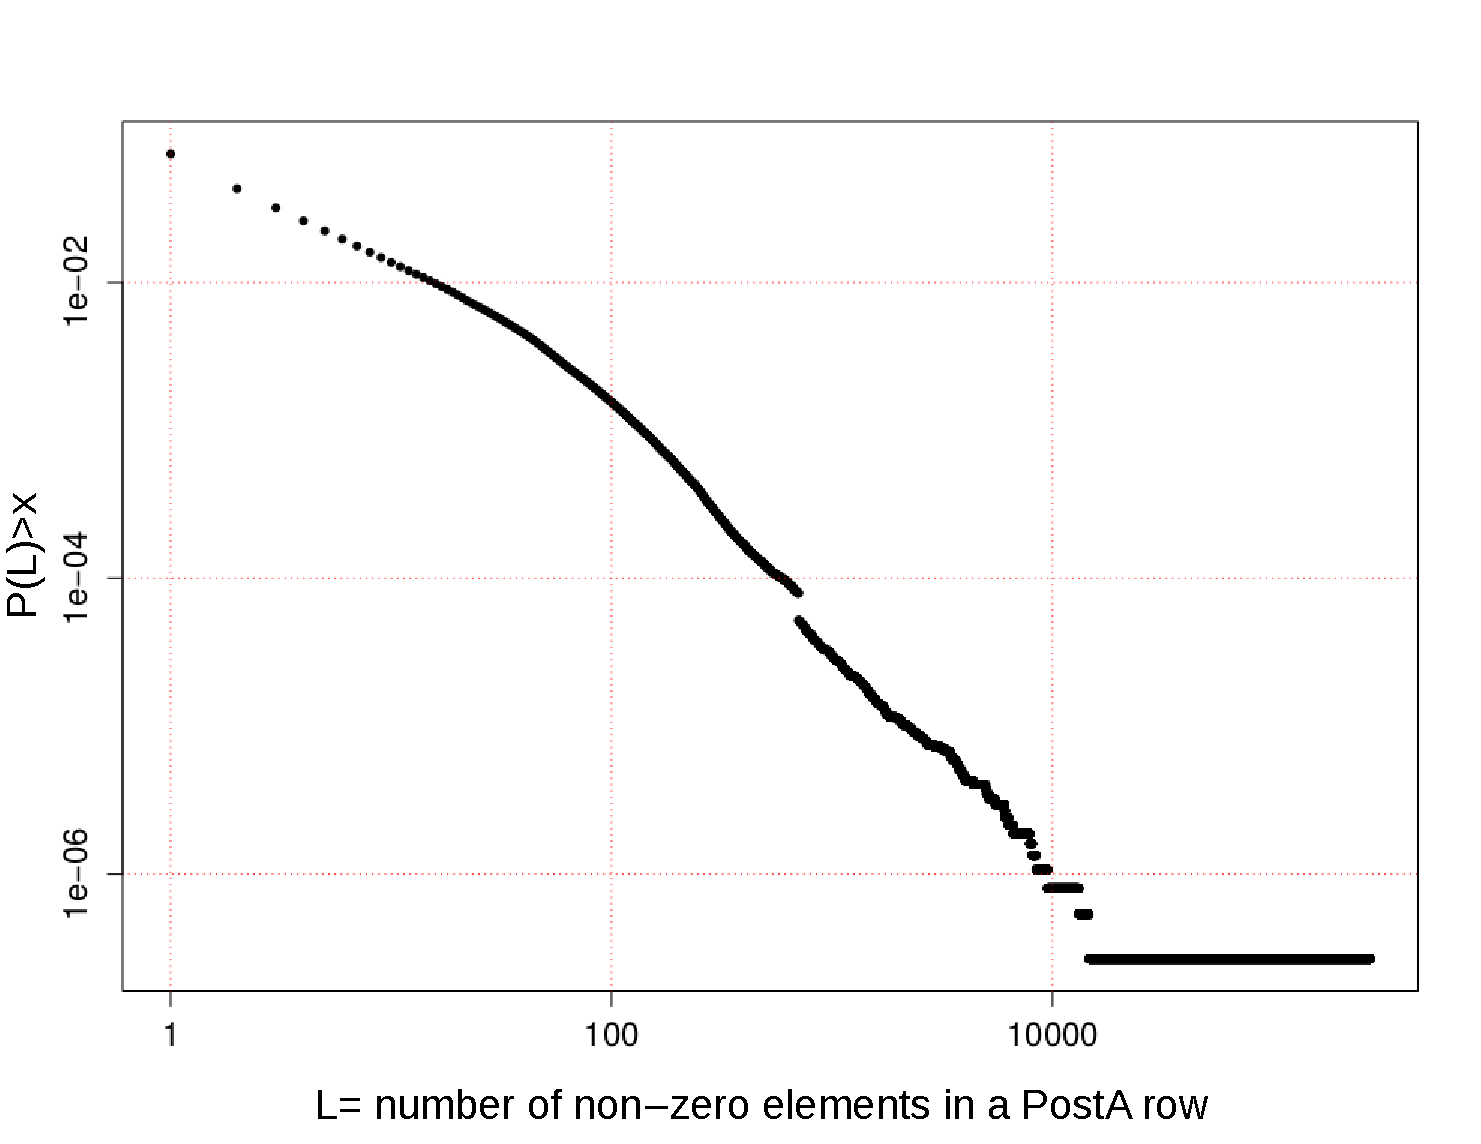
\includegraphics[width=0.95\linewidth]{PostA}
        \footnotesize
        \captionof{figure}{CCDF of $L$ for $\mathbf{PostA}$.}
        \label{fig_postA_CCDF}
    \end{minipage}
\end{frame}

\begin{frame}{Addresses Petri Net: Most Used and Imbalanced Addresses}
    \footnotesize
    \begin{block}{Usage Ranking}
        The most used addresses are identified by summing the nonzero elements in both $\mathbf{PreA}$ and $\mathbf{PostA}$ rows.
    \end{block}

    \begin{block}{Imbalanced Addresses}
        609,295 addresses show zero entries in $\mathbf{PreA}$ but at least one nonzero in $\mathbf{PostA}$. These addresses have never been used to spend bitcoins but only to receive them. Table~\ref{tab_imbalance_10addressPreA} lists the top 5 addresses by incoming transactions along with their current balances.
    \end{block}

    \begin{center}
        \begin{tabular}{cccc} %\toprule
            %\begin{tabular}{|c|c|c|c|}
            \hline
            Address                            & L post & current balance BTC \\ \hline
            15S1TFTosxrgZxkqJR2n1AFJ22ZJE2rTCk & 3,853  & 120.85215349        \\
            1PtnGiNvhAKbuUQ6nZ7nF3CDKCKGfeMsCX & 1,199  & 0                   \\
            129FTwWoi5H5ujasMZ6M6VjJzBJfsXVQGw & 1,138  & 0.78425567          \\
            1FN9kKsZA9XttrAwuDDgsXjs6CXUR2fzmt & 1,111  & 0                   \\
            1DYvtKtZ2Ay9vTjzjb9BiRauMgXdjRDaD  & 973    & 14.5601             \\
        \end{tabular}
        \vspace{.2cm}
    \end{center}
    \captionof{table}{Summary of first 5 most imbalanced addresses}
    \label{tab_imbalance_10addressPreA}

\end{frame}

\begin{frame}{Addresses Petri Net: Disposable Address Chains}
    \footnotesize
    \vspace{-0.2cm}

    \begin{itemize}
        \item \textbf{Disposable Addresses:} Defined as addresses used exactly twice (once to receive and once to send all bitcoins).
        \item Transactions involving disposable addresses typically have:
              \begin{itemize}
                  \item One pre-arc (single input) and two post-arcs (output to two distinct addresses).
              \end{itemize}
        \item The model easily identifies these by analyzing $\mathbf{PreA}$ and $\mathbf{PostA}$.
        \item 122,155 disposable address chains have been detected, involving 1,350,010 different addresses/transactions.
              % \item The longest chain recorded consists of 3,658 transactions.
    \end{itemize}
    \vspace{-0.2cm}
    \centering
    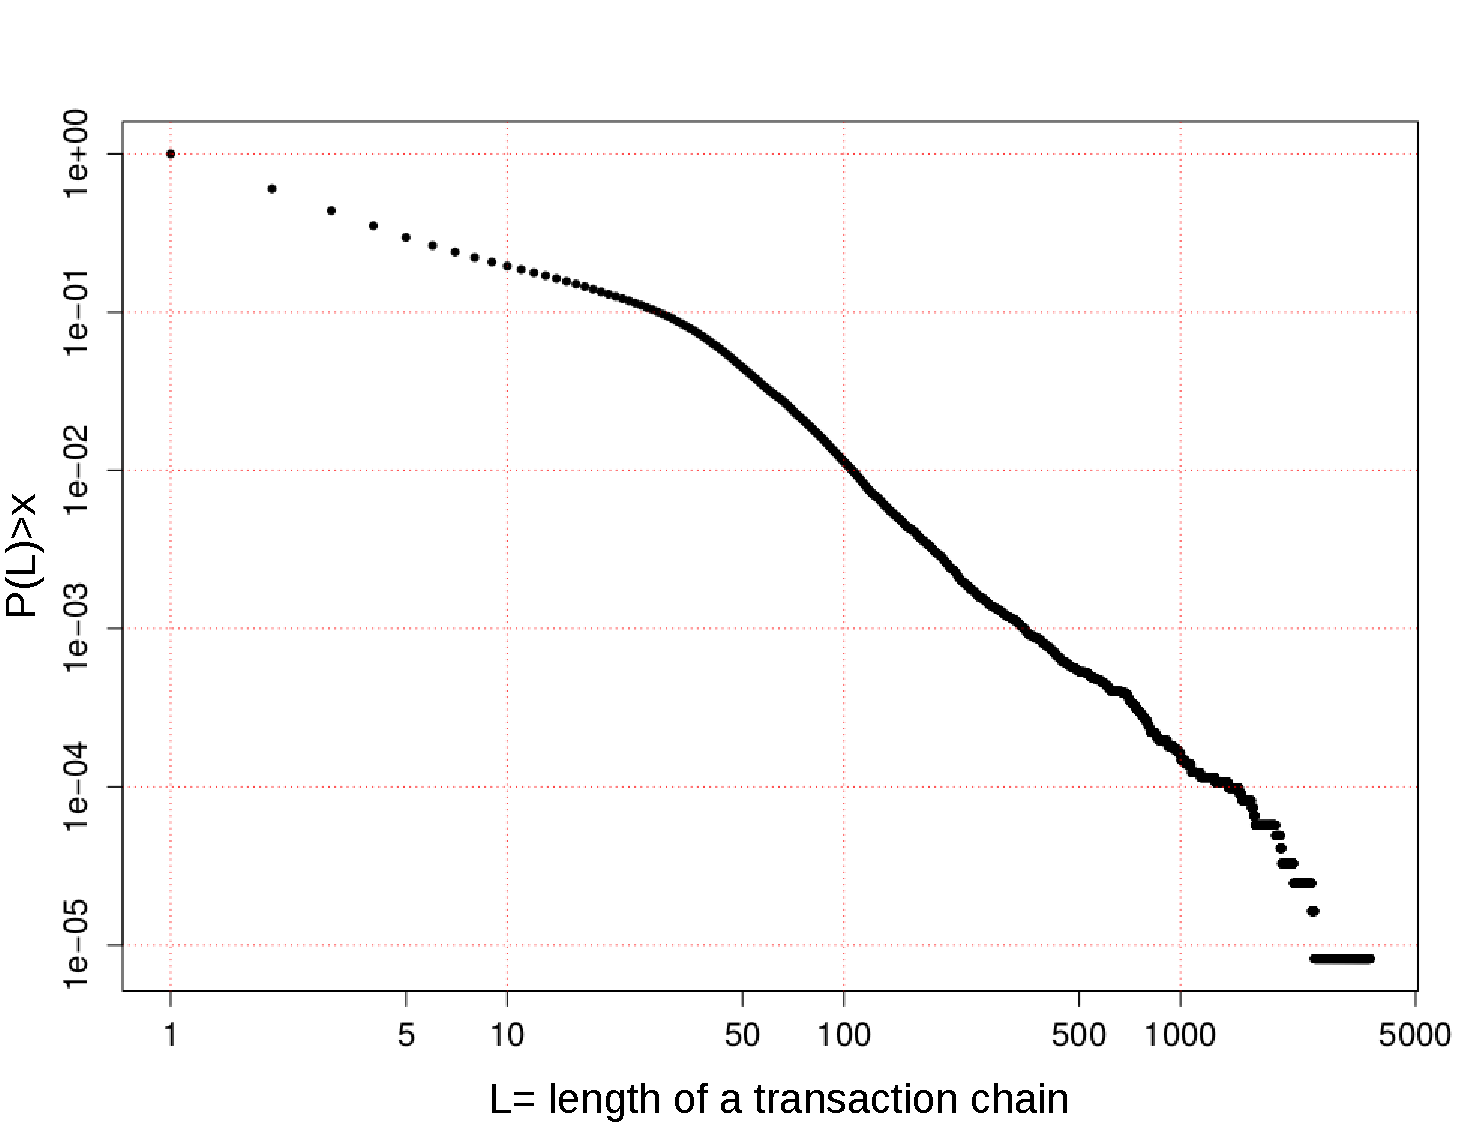
\includegraphics[width=0.5\linewidth]{Chains}
    \label{fig_chains_CCDF}
\end{frame}

\begin{frame}{Addresses Petri Net: Repeated Transaction Patterns}
    \footnotesize
    \vspace{-0.2cm}
    \begin{itemize}
        \item \textbf{Repeated Transfers:} Users sometimes execute transactions with identical sets of input and output addresses.
        \item In the Petri Net model, such repetitions appear as transitions with identical pre- and post-arc configurations.
        \item Approximately 11\% of transactions are repetitions, reflecting steady bitcoin flows between fixed groups of addresses.
        \item The CCDF of grouped transaction sizes (i.e., the number of repetitions) illustrates this phenomenon.
    \end{itemize}
    \vspace{-0.2cm}
    \centering
    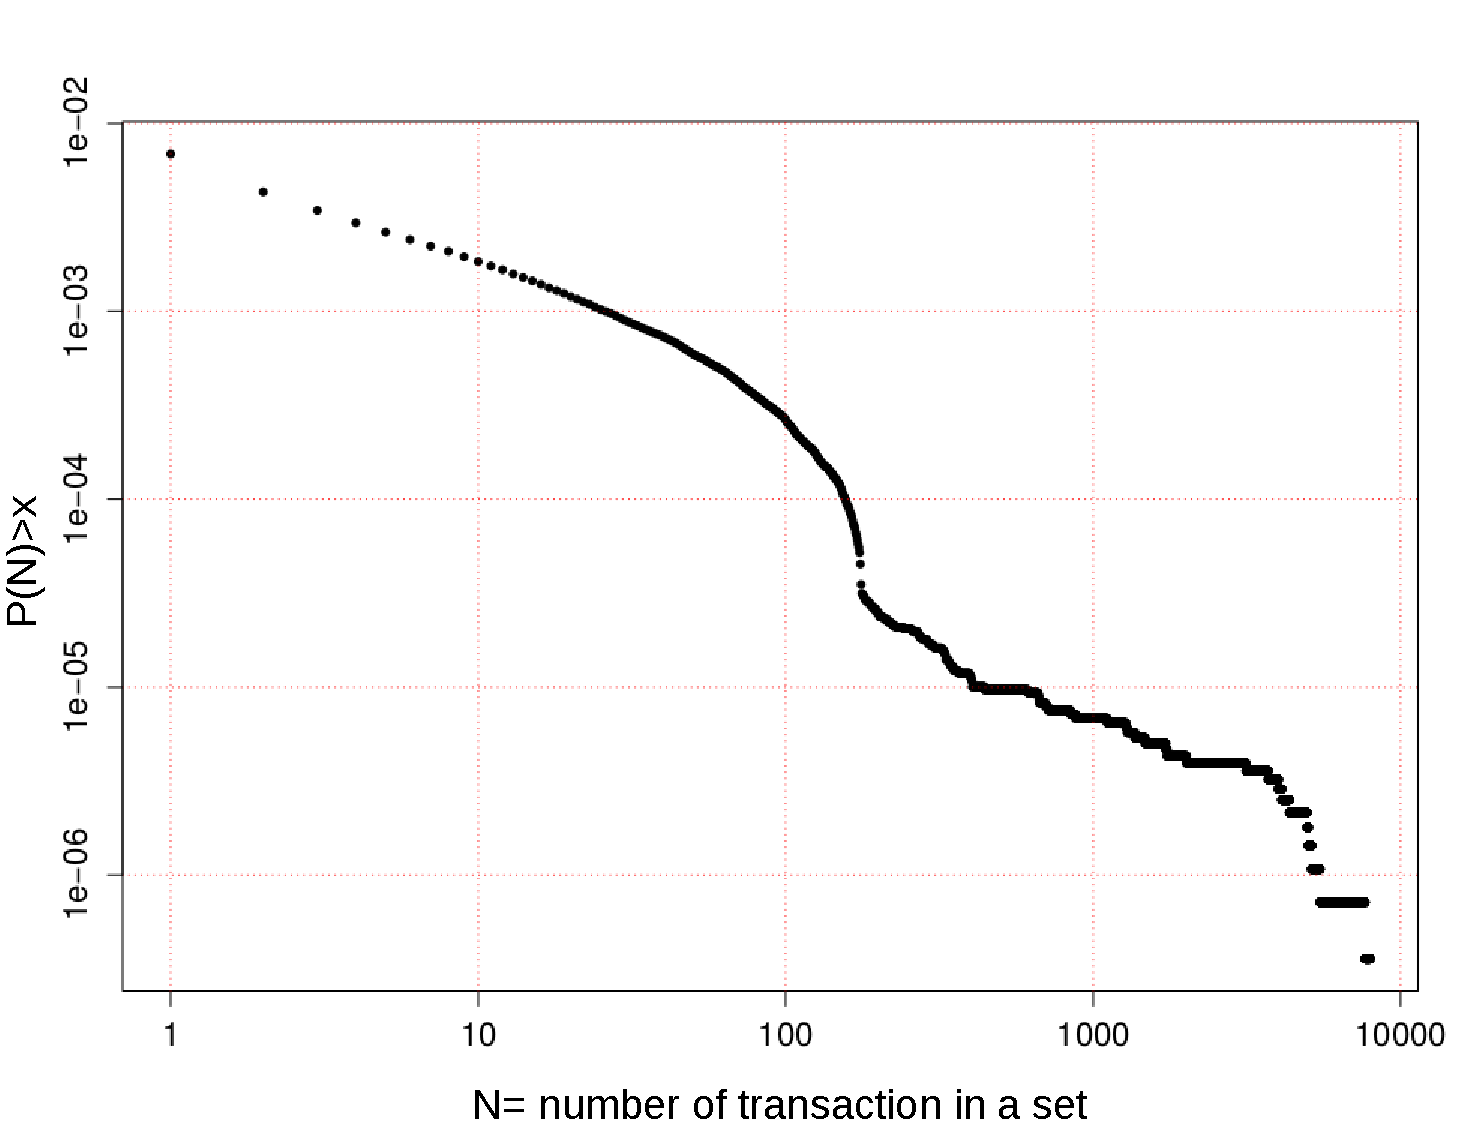
\includegraphics[width=0.5\linewidth]{groupTA}
    \label{fig_transA_CCDF}
\end{frame}

\subsection{Results of the Entities Petri Net}
\begin{frame}{Entities Petri Net: Address Distribution and Entity Control}
    \footnotesize
    \begin{itemize}
        \item \textbf{Entities and Addresses:} 2,461,010 entities control 3,730,480 addresses.
        \item Distribution is highly non-uniform and follows a power-law pattern:
              \begin{itemize}
                  \item Many entities hold a single address.
                  \item Few entities control a large number of addresses and influence a significant portion of bitcoin transactions.
              \end{itemize}
    \end{itemize}
    \vspace{0.3cm}
    \centering
    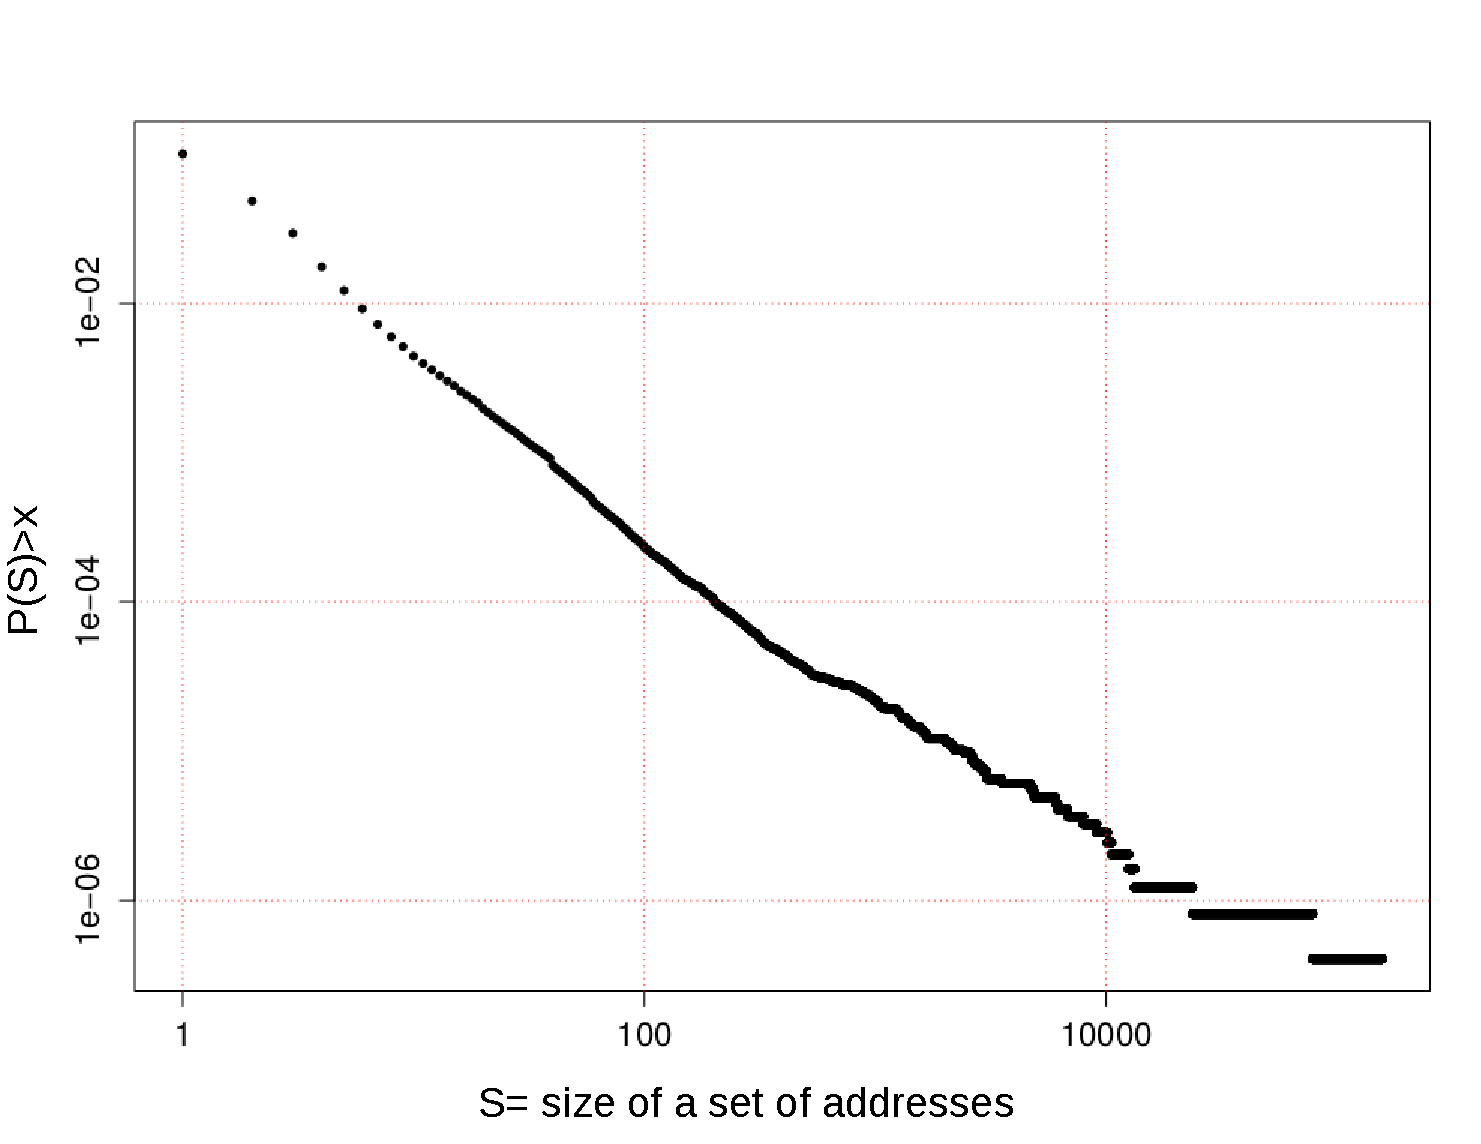
\includegraphics[width=0.6\linewidth]{Entity_size}
    \captionof{figure}{CCDF of the distribution of addresses across entities.}
    \label{fig_entity_CCDF}
\end{frame}

\begin{frame}{Entities Petri Net: Transaction Distributions for Entities}
    \footnotesize
    \begin{itemize}
        \item \textbf{Transaction Involvement:} The number of non-zero elements in the rows of $\mathbf{PreE}$ and $\mathbf{PostE}$ indicates how many transactions an entity is involved in.
        \item \textbf{Power-law Distribution:} Transactions among entities show a power-law behavior for both input and output transactions.
    \end{itemize}
    \vspace{0.3cm}
    \begin{minipage}[c]{0.45\textwidth}
        \centering
        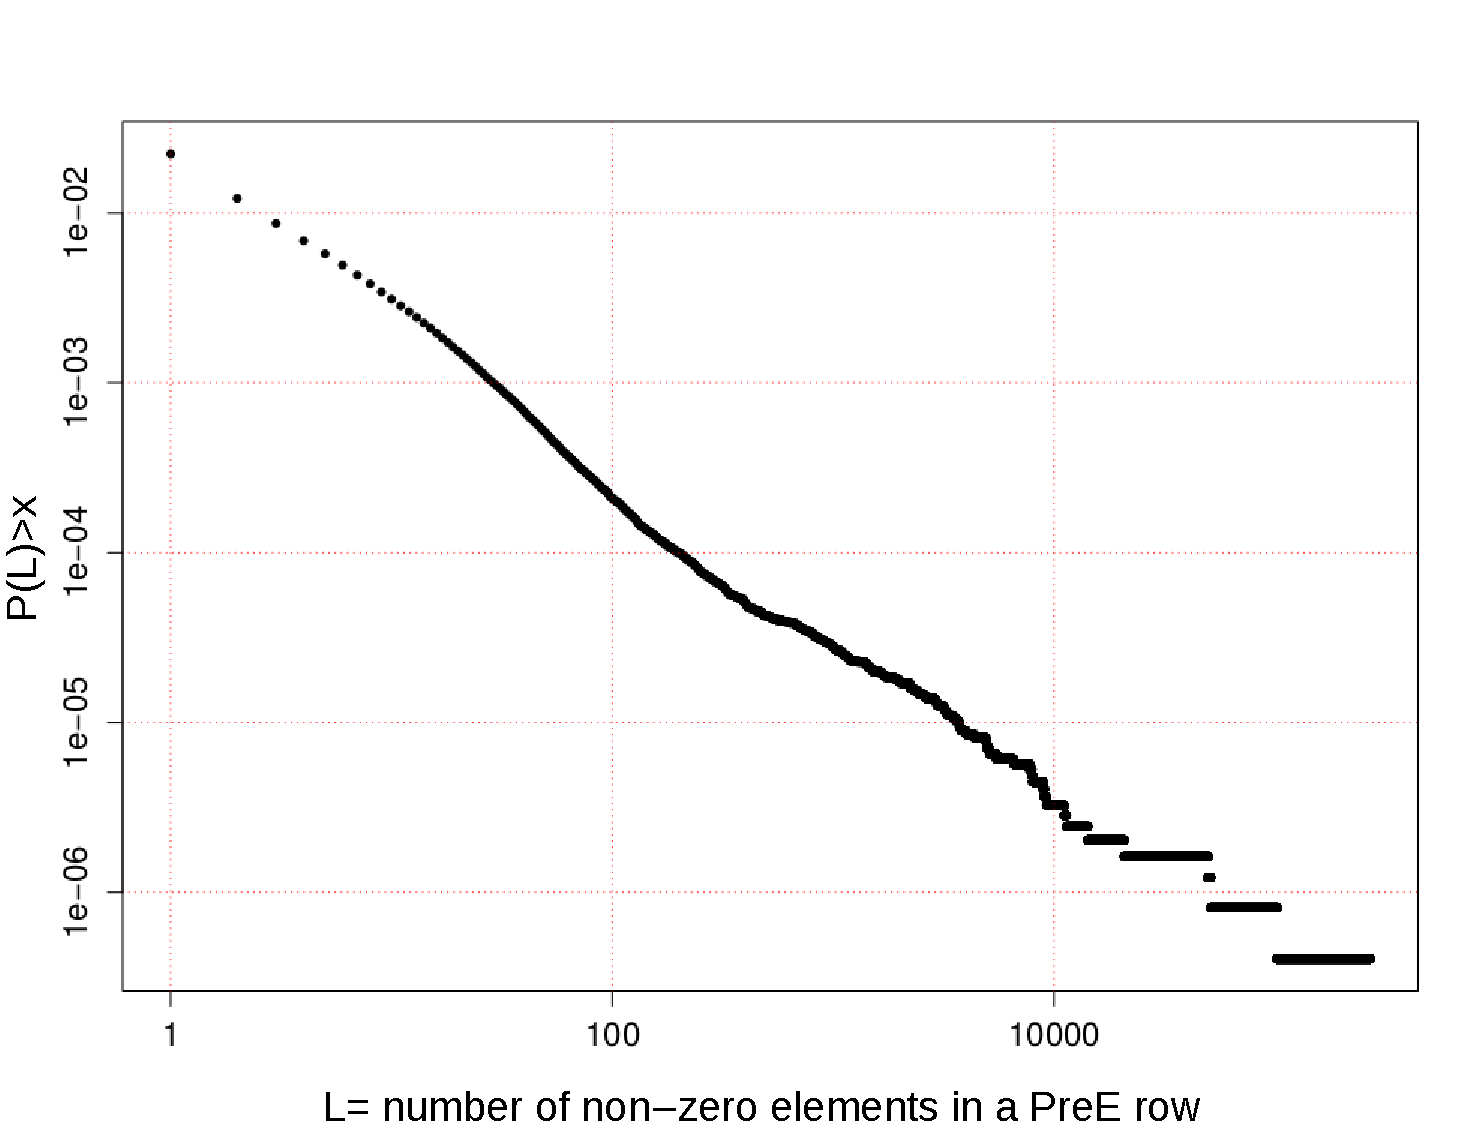
\includegraphics[width=0.95\linewidth]{PreE}
        \captionof{figure}{CCDF of the length $L$ for $\mathbf{PreE}$.}
        \label{fig_preE_CCDF}
    \end{minipage}
    \hspace{0.5cm}
    \begin{minipage}[c]{0.45\textwidth}
        \centering
        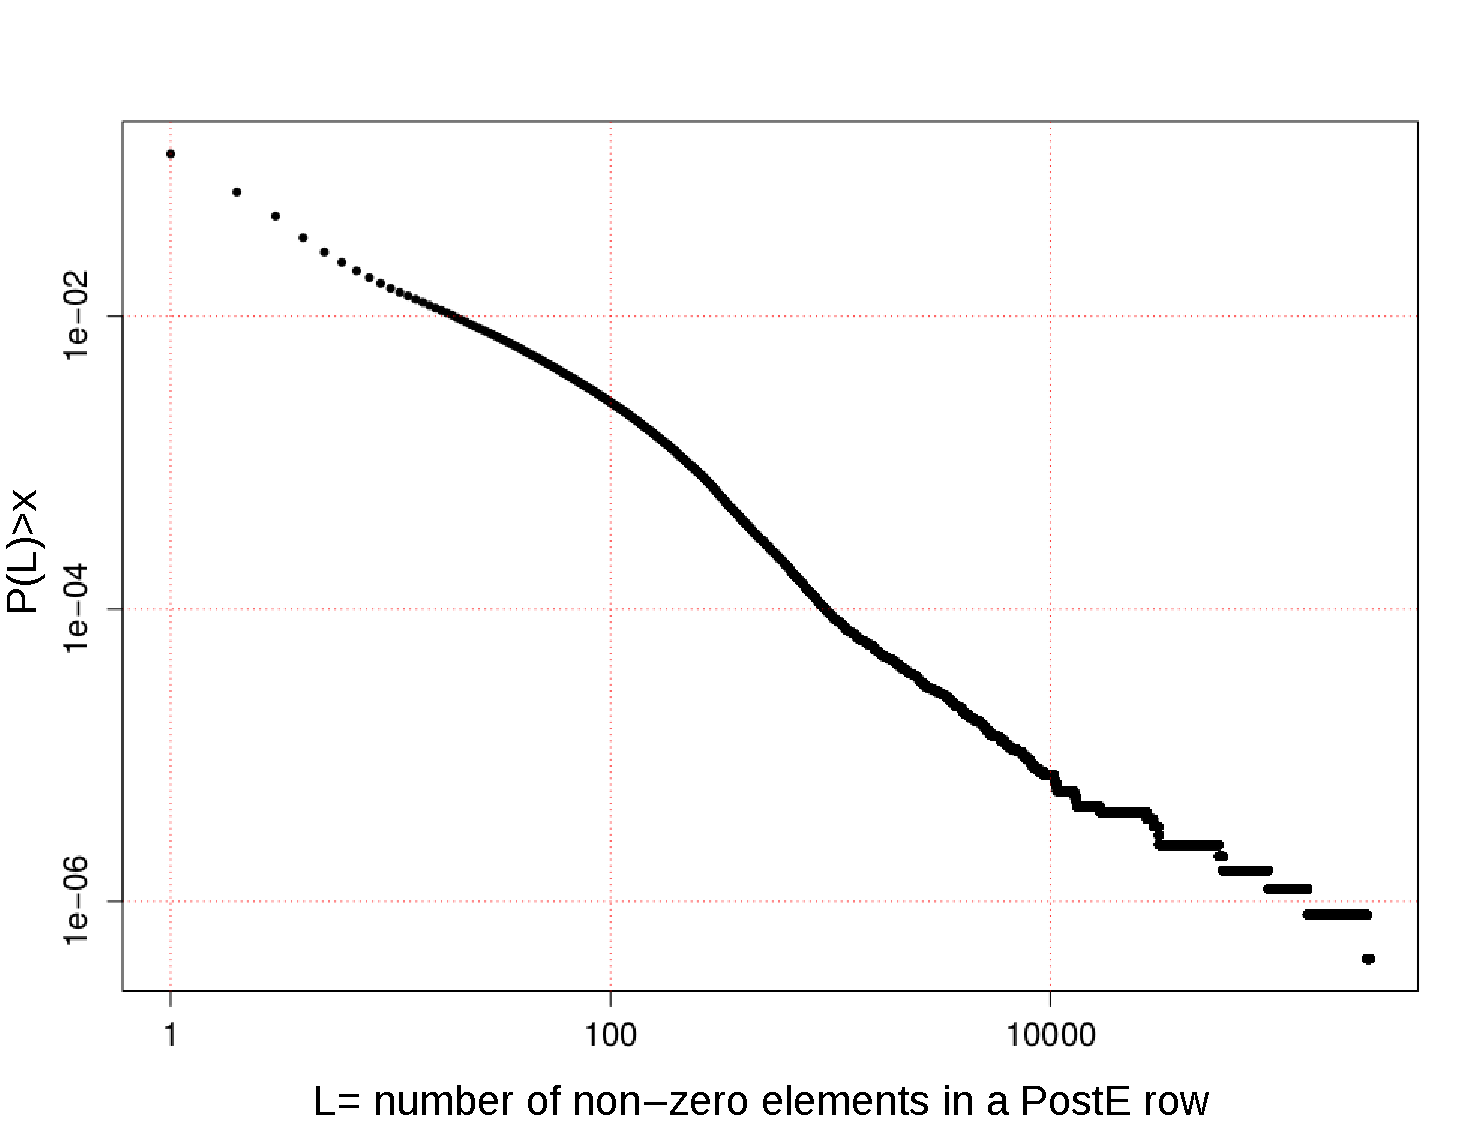
\includegraphics[width=0.95\linewidth]{PostE}
        \captionof{figure}{CCDF of the length $L$ for $\mathbf{PostE}$.}
        \label{fig_postE_CCDF}
    \end{minipage}
\end{frame}

\begin{frame}{Entities Petri Net: Most Active Entities}
    \footnotesize
    \begin{itemize}
        \item \textbf{Top Entities:} The 5 most active entities are identified by the sum of non-zero elements in both $\mathbf{PreE}$ and $\mathbf{PostE}$.
        \item Their balances are calculated by summing the balances of all addresses belonging to each entity.
        \item \textbf{Tags:} Some entities are associated with known tags (e.g., deepbit.net, ilovethebtc).
    \end{itemize}
    \vspace{-0.2cm}
    \begin{center}
        {\begin{tabular}{ccccc} %\toprule
                \hline
                Entity number & L pre   & L post  & size    & tags        \\ \hline
                95237         & 270,204 & 275,398 & 2       & deepbit.net \\
                2             & 102,186 & 283,973 & 156,725 & ilovethebtc \\
                37            & 51,228  & 147,712 & 78,251  & jmm5699     \\
                11            & 49,959  & 97,732  & 10,37   & - unknow -  \\
                130           & 20,857  & 58,350  & 23,649  & Instawallet \\
                \hline
            \end{tabular}}
        \vspace{.2cm}
        \captionof{table}{Summary of first 5 most active entities}
        \label{tab_10Entity_1}
    \end{center}
\end{frame}

\begin{frame}{Entities Petri Net: Repeated Transaction Patterns}
    \footnotesize
    \begin{itemize}
        \item \textbf{Repeated Transactions:} About 22.6\% of transactions are repetitions of previous transactions between the same input and output entities.
        \item These repetitions indicate steady fluxes of bitcoins at the entity level.
        \item \textbf{Visualization:} The CCDF for grouped transaction sizes demonstrates this repetitive behavior.
    \end{itemize}
    \vspace{-0.1cm}
    \centering
    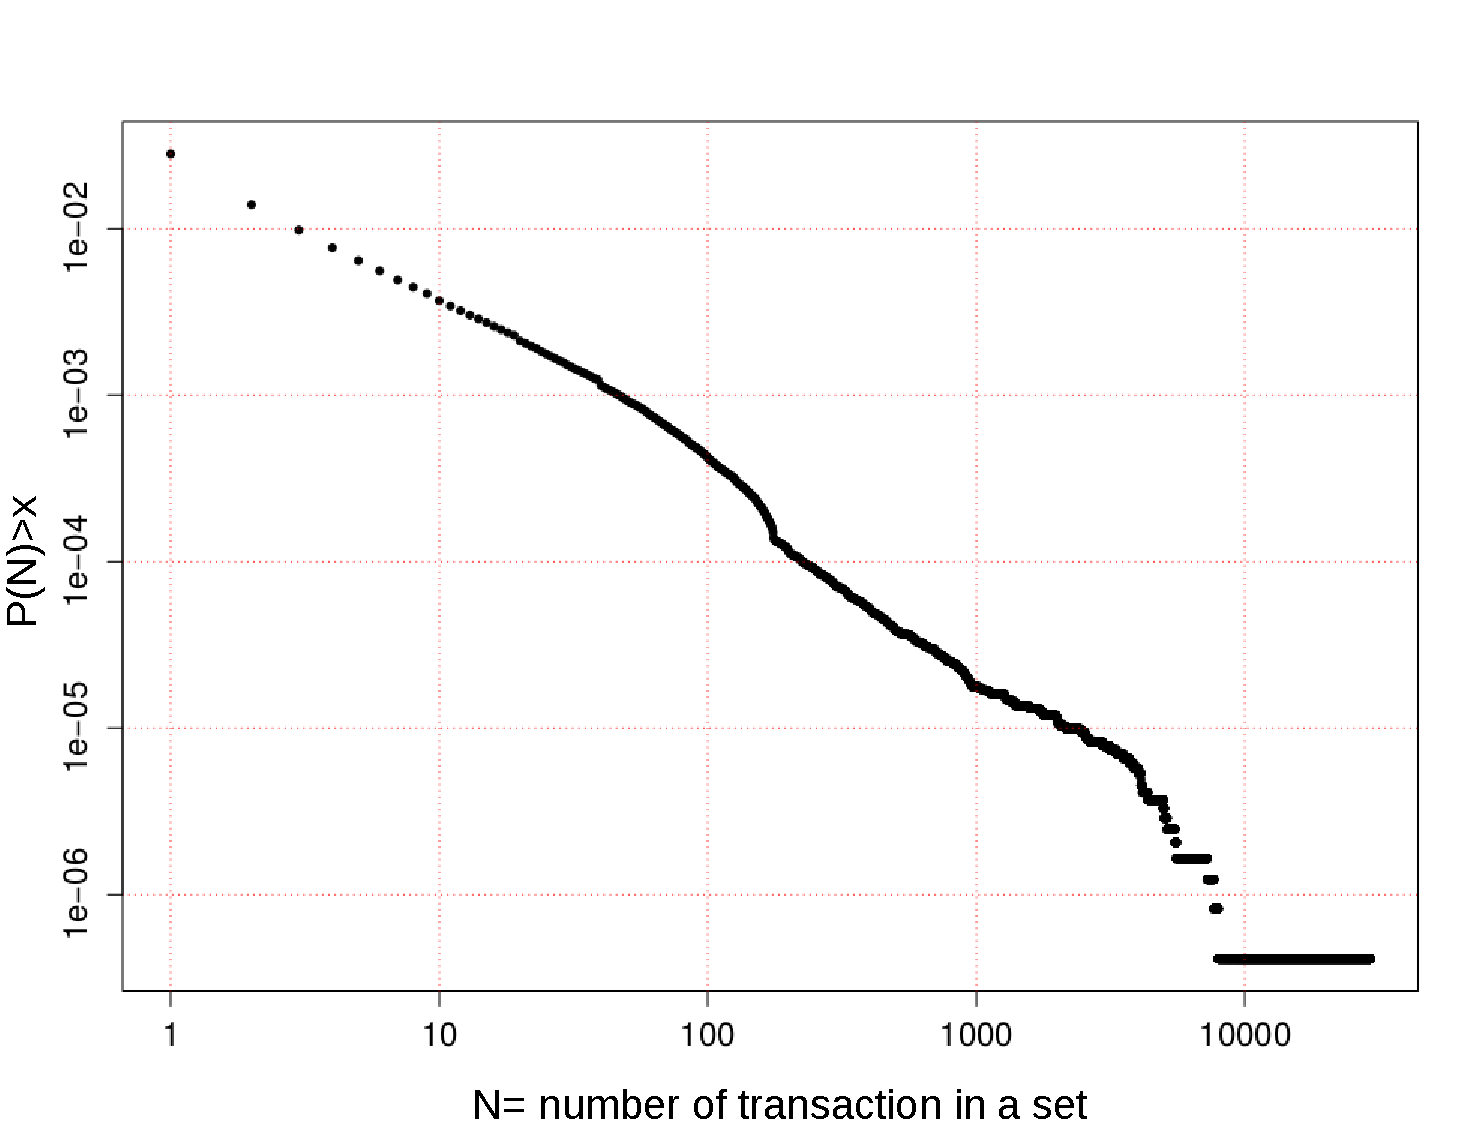
\includegraphics[width=0.5\linewidth]{groupTE}
    \captionof{figure}{CCDF of the size $L$ of grouped transaction sets for the Entities Petri Net.}
    \label{fig_transE_CCDF}
\end{frame}

\section{Analysis}
\begin{frame}{Analyzing Bitcoin Users with Petri Nets}
    \footnotesize
    \begin{block}{Petri Net Model}
        Clusters Bitcoin addresses into entities (246,660 owners control 1.5M addresses) and traces transaction chains (122,155 owners linked to 1.35M addresses).
    \end{block}

    \begin{block}{User Classification}
        368,815 engaged owners use disposable addresses or multiple addresses (72.6\% of transactions). 609,295 addresses are likely "deposit addresses" for engaged users.        255,045 addresses are owned by occasional users.
    \end{block}

    \begin{block}{Case Studies}
        Most active input address (270k transactions): \textit{DeepBit} mining pool (now defunct).
        Largest output entity (156k addresses): Tags include \textit{ilovethebtc}, \textit{mikeo}, and links to unreachable domains.
    \end{block}

    \begin{block}{Insight}
        Strongly uneven transaction distribution (CCDFs) suggests miner pools use high-activity addresses for reward redistribution.
    \end{block}
\end{frame}

\begin{frame}{Advantages of Petri Net Formalism}
    \footnotesize
    \begin{columns}[T]
        \begin{column}{0.45\textwidth}
            \vspace{-0.1cm}

            \begin{block}{Non-Deterministic Dynamics}
                Models UTXO-enabled transactions as independent events. Natively handles probabilistic block inclusion (miner fees, validation).
            \end{block}
            \vspace{-0.1cm}

            \begin{block}{Simulation Power}
                Captures concurrent non-conflicting transactions (e.g., same-block validations). Enables statistical modeling of future states (e.g., miner pool growth predictions).
            \end{block}
            \vspace{-0.1cm}

            \begin{block}{Sequential Analysis}
                Automatically identifies chains of disposable addresses (privacy-preserving flows).
            \end{block}
        \end{column}
        \begin{column}{0.45\textwidth}
            \vspace{-0.1cm}

            \begin{block}{Matrix-Driven Insights}
                Pre/Post matrices reveal never-spent addresses (609k output-only), single-use addresses, and transaction volumes.
            \end{block}
            \vspace{-0.1cm}

            \begin{block}{State Equations}
                Enable probabilistic forecasting of Bitcoin fluxes between entities (exchanges, pools) using historical data.
            \end{block}
        \end{column}
    \end{columns}
\end{frame}

\section{Conclusions}
\begin{frame}{Conclusions}
    \footnotesize
    \vspace{-0.1cm}

    \begin{block}{Novel Petri Net Architecture}
        Processed first 180,000 blocks ($\approx$ 3.5 years of Bitcoin history).\\[2mm]
        Addresses $\rightarrow$ Places (2.7M+), Transactions $\rightarrow$ Transitions.\\[2mm]
        Pre/Post matrices capture all input-output relationships.
    \end{block}
    \vspace{-0.1cm}

    \begin{block}{Key Discoveries}
        Universal power-law distributions were observed in transaction arcs (pre/post connections), disposable address chain lengths, and repeated input-output transaction clusters.\\[2mm]
        Entity Network Reconstruction: Built a secondary Petri Net of address owners through matrix analysis.
    \end{block}
    \vspace{-0.1cm}

    \begin{block}{Computational Considerations}
        The current blockchain (480k+ blocks, 240M+ transactions) challenges full-scale analysis.\\[2mm]
        Flexible partial analysis allows investigation of specific address subsets or time windows.
    \end{block}
\end{frame}

\end{document}
